% !TEX encoding = UTF-8 Unicode

\documentclass[12pt,oneside]{amsart}
\usepackage{cancel}
\usepackage{xspace}
\usepackage{graphicx}
\usepackage{multicol}
\usepackage{subfig}
\usepackage{amsmath}
\usepackage{amssymb}
\usepackage[a4paper,width=165mm,top=20mm,bottom=25mm,includeheadfoot]{geometry}
\usepackage{array}
\usepackage{verbatim}
\usepackage{caption}
\usepackage{natbib}
\usepackage{float}
\usepackage{pdflscape}
\usepackage{mathtools}
\usepackage[usenames,dvipsnames]{xcolor}
\usepackage{afterpage}
\usepackage{tikz}
\usepackage[bookmarks=true, unicode=true, pdftitle={Nexty Yellow Paper: a formal specification of Nexty, a zero transfer fee and instant transfer base on Ethereum blockchain}, pdfauthor={Thanh Dao / Ha Dang},pdfkeywords={Nexty, Ethereum, Yellow Paper, blockchain, virtual machine, cryptography, decentralised, singleton, transaction, generalised, zero transfer fee, instant transfer},pdfborder={0 0 0.5 [1 3]}]{hyperref}
%,pagebackref=true

\PassOptionsToPackage{hyphens}{url}\usepackage{hyperref}

\makeatletter
 \newcommand{\linkdest}[1]{\Hy@raisedlink{\hypertarget{#1}{}}}
\makeatother
\usepackage{seqsplit}

% For formatting
%\usepackage{underscore}
%\usepackage{lipsum} % to generate filler text for testing of document rendering
\usepackage[english]{babel}
\usepackage[autostyle]{csquotes}
\MakeOuterQuote{"}

\definecolor{pagecolor}{rgb}{1,0.98,0.9}

%Path relative to the main .tex file 
\graphicspath{ {./images/} }

\title{NEXTY: A CONSENSUS TO GET ZERO TRANSFER FEE AND INSTANT TRANSFER BLOCKCHAIN}
\author{
	Thanh Dao \& Ha Dang \\
	CO-FOUNDER/CTO NEXTY PLATFORM \\
	thanhdao@nexty.io / dvietha@gmail.com
}
\date{} % delete this line to display the current date

%%% BEGIN DOCUMENT
\begin{document}

\pagecolor{pagecolor}
\begin{abstract}
Đây là phần mô tả mang tính kỹ thuật của Nexty Platform, tập trung vào việc chi tiết cách thức vận hành của Consensus Protocol tên là Proof of Foundation (Algorithm name: DCCS - Dual Cryptocurrency Confirmation System). Proof of Foundation được inspired từ Proof of Authority được đề xuất bởi \cite{clique}, nhưng vận hành theo DCCS để có được tính decentralized hoàn thiện hơn và đồng thời mang lại sự incentive cho những người duy trì blockchain.
\end{abstract}

\maketitle

\setlength{\columnsep}{20pt}
\begin{multicols}{2}
%\tableofcontents

\section{Mô tả chung}\label{sec:introduction}
DCCS là hệ thống có thêm 1 token thứ 2 tên là NTF ngoài NTY. NTF là token dùng để xác định Authorities duy trì confirmation system, đồng thời cũng xác định số lượng trả thưởng cho việc đóng Blocks. NTF là token có số lượng 10,000,000 được tặng tương ứng với 100,000,000,000 NTY đầu tiên tham gia chương trình smart staking đã được mô tả chi tiết trong whitepaper của \cite{smart-taking}, hay có thể nói là những người đầu tiên có tầm nhìn và tâm huyết với hệ thống của Nexty. Chính vì thế consensus protocol được đặt tên là Proof of Foundation. Tuy nhiên, sức mạnh của hệ thống lại không nằm ở những người sở hữu NTF vì họ có thể bị vote down trong những trường hợp như phát hiện gian lận, quá centralized, hay không cập nhật kịp thời source code mới từ hệ thống. Chính vì vậy, ở một khía cạnh khác có thể nói những người sở hữu NTF là những người đi làm thuê cho hệ thống, và bản thân họ không phải là những người chủ thực sự của Nexty blockchain. Đây là một decentralized system mới, được duy trì bởi cộng đồng người dùng sở hữu NTY.

\section{Cách thức authorize một account được trở thành block sealer}
Hệ thống sẽ đặt ra một config parametter để xác định giá trị tối thiểu min-ntf mà một địa chỉ NTF cần phải có để có thể trở thành block sealer.
Nexty sẽ xây dựng và phát triển một smart contract, trong đó chỉ định gán quyền của một địa chỉ NTF với số lượng token lớn hơn min-ntf, sang một địa chỉ Account khác gọi là executing-account với giá trị state là authorized-sealer với giá trị bằng địa chỉ của NTF. Nếu một địa chỉ đã tồn tại một giá trị authorized-sealer thì nó ko thể nhận authorization từ một NTF holder nào khác cho đến khi NTF holder đó tạo lệnh withdraw từ authorized-sealer. Lệnh đặt authorized-sealer phải được thực hiện sau khi cài đặt và vận hành sealing node bằng cách đọc state từ smart contract để có thể xác định danh sách authorized-sealer được tham gia vào sealing round tiếp theo. Trường hợp nếu trong sealing round hiện tại, authorized-sealer không thực hiện 1 sealing activity thì giá trị authorized-sealer sẽ bị withdraw về NTF holder của nó bằng cách thay đổi state của smart contract tại checkpoint block number của sealing round tiếp theo và tất nhiên authorized-sealer đó sẽ không được tham gia vào sealing round tiếp theo cho đến khi được authorize trở lại.

\section{Cách thức các sealers đóng block}
Cách thức đóng Block của DCCS là các sealers sẽ được đánh số từ $1$ đến $n$ (gọi là ``sealing-id'') một cách ngẫu nhiên theo từng sealing round: trong đó $n$ là số lượng các authorized-sealers đã được đăng ký và được xác định từ state của smart contract tại checkpoint block number của sealing round tương ứng. Để đảm bảo tính ngẫu nhiên khi đánh số ``sealing-id'', thì việc đánh số theo mã hash, $\boldsymbol{\xi_{\mathrm{k}}}$, được tính toán theo công thức sau đây khi bắt đầu một sealing round mới. 
\begin{equation}
\xi_{\mathrm{k}} \equiv \texttt{\small KEC}(\mathbf{block}, \mathbf{\Lambda_{\mathrm{k}}})
\end{equation}

\begin{description}
\item[block] là block number đầu tiên, a.k.a checkpoint block number, của sealing round
\item[$\Lambda_{\mathrm{k}}$] là địa chỉ ví mà NTF holder đã thiết định để làm authorized-sealer trong smart contract.
\item[\texttt{\small KEC}] là hàm tính băm của một input bất kỳ theo thuật toán \textbf{SHA-3 Keccak-512}.
\end{description}

Sau đó, ``sealing-id'' của từng authorized-sealer sẽ được lấy bằng vị trí của \textit{sealing hash}, $\boldsymbol{\xi_k}$, trong array $(\xi_{\mathrm{1}}, \xi_{\mathrm{2}}, ..., \xi_{\mathrm{n}})$ đã được sắp xếp theo thứ tự tăng dần theo \textit{sealing hash} của toàn bộ các authorized-sealers tại sealing round hiện thời.

Để đảm bảo performance của hệ thống thì ``sealing-id'' của toàn bộ authorised sealer sẽ được snapshot duy nhất một lần từ state của smart contract tại checkpoint block number của mỗi sealing round và lưu vào \textbf{lru cache} của từng node.

\subsection{Trường hợp 1} Nếu sealing node không nằm trong recent sealers. Node sẽ xác định block tiếp theo có phải là đến lượt nó làm sealer hay không theo công thức sau:

\begin{equation}\label{eq:sigma}
\sigma_{\mathrm{k}} \equiv (\nu - \mathbf{block}) \ \ \ \mathbf{mod} \ \ \ \Pi
\end{equation}

\begin{description}
\item[$\nu$] là block number hiện tại sẽ được seal.
\item[block] là block number đầu tiên, a.k.a checkpoint block number, của sealing round
\item[$\Pi$] tổng số authorised sealer đã được xác định tại checkpoint block của sealing round hiện tại.
\end{description}

Nếu số dư $\sigma_{\mathrm{k}}$ bằng chính ``sealing-id'' của node thì node đó được quyền seal block ngay lập tức. Đối với số dư khác với ``sealing-id'', ở mỗi block tiếp theo, các sealing node phải tự xác định thời gian chờ, $\psi_{\mathrm{k}}$, được tính như sau:

\begin{eqnarray}
\alpha = 001.387978000 \\
\beta = 000.002313279 \\
\gamma = 000.004626590 \\
\delta = 199.999400000
\end{eqnarray}

\begin{equation}\label{eq:psi}
\psi_{\mathrm{k}} \equiv \sum_{i=1}^{\zeta_\mathrm{k}} \mathbf{floor}(\frac{\alpha}{\beta*i+\gamma} + \delta)
\end{equation}

\subsection{Trường hợp 2} Nếu sealing node nằm trong recent sealers

Trường hợp này có thể cho sealers được tiếp tục seal, nhưng phải đợi hết 1 vòng khi không còn sealer không nằm trong recent sealers đang hoạt động. Đây là phương thức nhằm đảm bảo khi chỉ còn 1 sealer thì hệ thống vẫn có thể tạo block, tuy nhiên với thời gian rất lâu. Thời gian này rơi vào khoảng 3 - 30 phút nếu có từ 1000 - 10,000 authorized sealers nhưng chỉ có một hoặc rất ít active sealers.

Thời gian chờ $\psi_{\mathrm{k}}$ được theo công thức sau:

\begin{eqnarray}
\alpha = 001.387978000 \\
\beta = 000.002313279 \\
\gamma = 000.004626590 \\
\delta = 199.999400000
\end{eqnarray}

\begin{multline}\label{eq:psi_2}
\psi_{\mathrm{k}} \equiv \sum_{i=1}^{n} \mathbf{floor}(\frac{\alpha}{\beta*i+\gamma} + \delta) \\ 
+ \sum_{i=1}^{\zeta_\mathrm{k}} \mathbf{floor}(\frac{\alpha}{\beta*i+\gamma} + \delta)
\end{multline}

Cách thức xây dựng hệ số cho công thức trên được giả định như sau. Đối với sealing node có sealing-id trùng với số dư r, được tính theo công thức $\eqref{eq:sigma}$, thì được ưu tiên seal block trước 400ms, sealing node tiếp theo được ưu tiên 350ms, và sau đó lần lượt là 320… cho đến sealing node lớn hơn số dư một khoảng lớn nhất thì xấp xỉ 200ms. Đồ thị của nó sẽ tương ứng với hàm số $\texttt{\small y} = \frac{a} {(b * x + c)} + \texttt{\small d}$

Để ước lượng giá trị cho các tham số của công thức này, chúng tôi sử dụng phương pháp curve fitting để tìm ra hệ số tương đối theo website \href{https://mycurvefit.com/}{My Curve Fit} với phương sai \footnote{R² is 1 minus the ratio of sum of the squares of the residuals divided by the sum of the squares of the differences between Y fit and the mean Y value} xấp xỉ bằng 1.
\\
\\
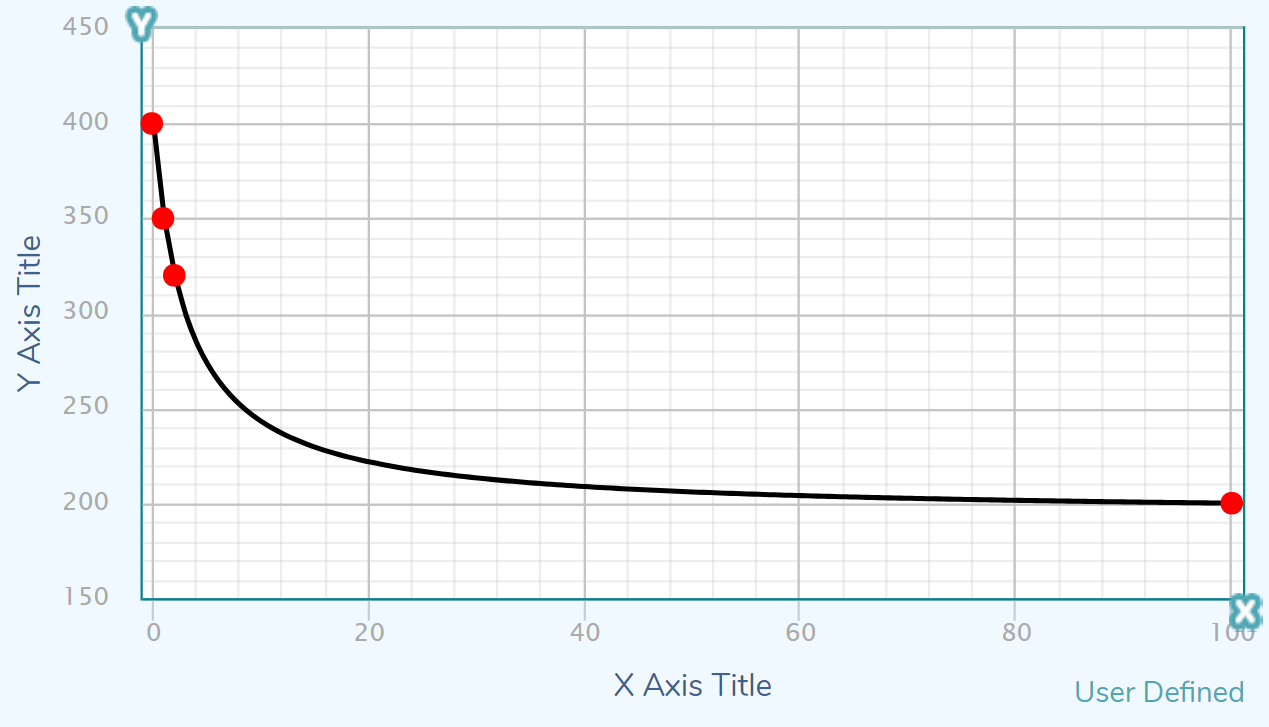
\includegraphics[width=0.48\textwidth, height=4cm]{curve-fit}
\\
Mỗi một vòng đóng block của các sealers sẽ được gọi là một epoch. Tuỳ theo số lượng sealer trong chain của từng sealing round mà một epoch sẽ có độ dài khác nhau.

Bằng phương thức tính thời gian chờ cố định cho từng sealers theo công thức  $\eqref{eq:psi}$ và $\eqref{eq:psi_2}$, consensus có thể kiểm tra được xem một sealer; vì lo ngại bị withdraw authorised sealer về NTF holder do không thực hiện sealing activity trong một sealing round mà chiếm quyền sealing block tại một thời điểm nào đó sớm hơn khi chưa đến lượt seal; gây ra sự hỗn loạn và racing for sealing block. Thuật toán đồng thuận của Nexty sẽ thực hiện verify một block được seal bởi một authorized sealer bằng cách kiểm tra lại xem thời gian sinh ra block của authorized-sealer đó có đúng nhỏ hơn thời gian nó phải chờ hay không.

\section{Cách thức trả thưởng cho các sealers}

Cứ sau mỗi sealing round, giá trị thưởng $\Re$ của mỗi sealer sẽ được tính bằng giá trị nhỏ nhất của tổng số lượng thưởng chia cho các active sealers theo tỷ lệ số lượng NTF họ có trên tổng số NTF của những người được làm sealers mà có tham gia quá trình seal.

\begin{eqnarray}
\theta = \frac{\Omega}{N} \\
\phi = \frac{\Upsilon_{NTF}}{\Xi_{NTF}}
\end{eqnarray}

\begin{equation}\label{eq:re}
\Re \equiv \mathbf{min}(\theta, \phi)
\end{equation}

\begin{description}
\item[$\Omega$] total reward
\item[N] total number of active sealer of the current sealing round
\item[$\Upsilon_{NTF}$] amount of NTF token that the owner of active sealer is holding
\item[$\Xi_{NTF}$] total amount of NTF token that all active sealer are holding
\end{description}

Bằng cách thức tính reward $\Re$ theo công thức $\eqref{eq:re}$, người sở hữu nhiều NTF theo một cách tự nhiên sẽ phân chia NTF của mình ra nhiều ví để trang bị nhiều máy làm sealer, thay vì chỉ build một máy sealer và tập trung quá nhiều NTF vào đó. Điều này đảm bảo Nexty chain sẽ có số lượng node đủ lớn để đảm bảo tính decentralise, tính ổn định và tăng độ chịu tải cho toàn bộ Nexty chain.

Total reward $\Re$ là lượng NTY được sinh ra sau mỗi 1 sealing round, được tính bằng \textit{[số reward sinh ra 1 block]} * \textit{[số block được tạo ra ở sealing round đó]}

Số reward sinh ra cho một block được bằng số reward trong một năm chia cho $\mathbf{15768000}$, số block dự kiến trong vòng một năm với block time được config ban đầu của Nexty chain là 2 giây.

Số lượng reward sinh ra trong một năm được tính theo tỷ lệ sau đây:

\begin{center}
  \begin{tabular}{@{} cc @{}}
    \hline
    Year &  \% of circulating supply \\ 
    \hline
    1 & 10 \\ 
    2 & 5 \\ 
    3 & 2 \\ 
    4 & 1 \\ 
    5 & 1 \\     
    ... & ... \\ 
    ... & ... \\ 
    ... & ... \\ 
    n &  1 \\
    \hline
  \end{tabular}
\end{center}

\section{Cách thức chống SPAM hệ thống}

Do transaction fee của Nexty là zero nên nếu không có phương thức chống Spam transaction hợp lý thì dễ dàng có thể bị tấn công bằng cách gửi liên tục nhiều giao dịch trong cùng 1 lúc gây ra nghẽn hệ thống.

Chúng tôi đã có phương thức chống spam như sau:

Nguyên tắc chung là hệ thống sẽ thu phí ở giao dịch đầu tiên với mức phí khoảng \textit{0.2 USD/1 tài khoản}, số tiền này sẽ được cộng vào giá trị reward của sealing round. Từ những giao dịch sau đó, hệ thống sẽ không thu phí giao dịch, nhưng yêu cầu các tài khoản đó phải chạy ứng dụng ví liên tục với số lượng block bằng \textit{[0.0015 * gas-used]} thì mới được gửi giao dịch tiếp theo.

Ứng dụng ví của người dùng là một bản light client hay còn gọi là một block verifier (theo chuẩn light client protocol) có chức năng lưu lại những transaction của chính tài khoản đó, những tài khoản bên cạnh trong merkle tree, block number và các block header. Nhiệm vụ của light client là phải verify toàn bộ các thông tin giao dịch liên quan đến nó, cũng như xác thực tính đúng đắn của các block đã được sinh ra và block được sinh ra sau đó. Phải có 1 sự so sánh nếu blockchain bị can thiệp quá 15 block trở về trước thì phải có thông báo tới owner của ví đó rằng có thể hệ thống bị manipulated. Trong trường hợp đó sẽ cần truy cập cộng đồng chung để xem có lỗi nào xảy ra, đồng thời vote down đối với những authorized-sealers đã gây ra tình trạng sai sót đó.

Với nguyên tắc này, một hành động spam phải bỏ ra một lượng tài nguyên hệ thống của nó lớn hơn khoảng 56.7 lần lượng tài nguyên của chain để xác nhận một giao dịch như vậy sẽ làm cho những đối tượng spammer tổn thất nhiều hơn và không còn ý định spam.

Người dùng vẫn có quyền lựa chọn tạo transaction mất phí trong trường hợp họ không muốn duy trì block verifier như thế.

Đối với những dApp, nó có thể tự cung cấp các hệ thống nodes để chịu phần gas của người dùng rồi sau đó có thể có hoặc không thu phí trên phần gas của người dùng tuỳ theo nhu cầu phát triển của dApp đó.


\bibliographystyle{plainnat}
\bibliography{Biblio}

\end{multicols}
\end{document}